\newaufgabe{Erklären sie (und rechnen sie ein konkretes Beispiel durch), 
wie modulare Inversion
mit dem erweiterten Euklidischen Algorithmus realisiert werden kann.}
Der erweiterte euklidische Algorithmus berechnet für zwei Zahlen $a,b\in\mathbb{N}$
den größten gemeinsamen Teiler $\gcd(a,b)$. Außerdem liefert der Algorithmus zwei
weitere Zahlen $s,t\in\mathbb{Z}$, sodass der größte gemeinsame Teiler als Linearkombination
dieser Zahlen geschrieben werden kann (Lemma von Bézout).
\[
    \gcd(a,b) = s\cdot a + t \cdot b
\]
Das modulare Inverse einer Zahl $a\in \mathbb{N}$ ist eine Zahl $x\in\mathbb{Z}_n$, sodass
\[
    a\cdot x \equiv 1 \mod n.
\]
Um $x$ zu bestimmen, berechnet man zuerst über den erweiterten euklidischen Algorithmus
das Tupel $(\gcd(a, n), s, t)$. Ein modulares Inverses existiert genau dann, wenn
$\gcd(a,n) = 1$ (also $a$ und $n$ teilerfremd sind). Nach dem Lemma, lässt sich
der größte gemeinsame Teiler dann wie folgt schreiben.
\begin{align*}
    \gcd(a,n) = 1 &= s\cdot a + t\cdot n\\
    1 &\equiv s\cdot a + t\cdot n\mod n\\
    1 &\equiv s\cdot a\mod n
\end{align*}
Somit ist $s$ das modulare Inverse zu $a$ modulo $n$.
\paragraph{Algorithmus} Pseudocode des erweiterten euklidischen Algorithmus
\footnote{\href{https://de.wikipedia.org/wiki/Erweiterter_euklidischer_Algorithmus\#Rekursive_Variante}{Wikipedia, rekurisver, erweiterter euklidischer Algorithmus}}
\begin{figure}[h]
    \centering
    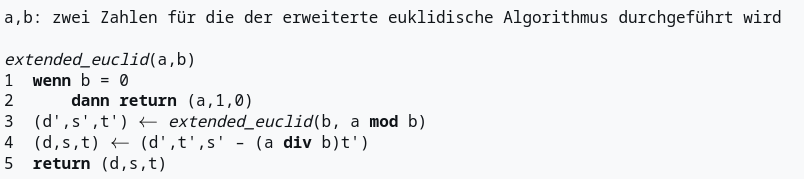
\includegraphics[width=\textwidth]{img/extended_euclid.png}
    \label{ref:ext_euclid}
\end{figure}\newpage
\begin{example}
    Seien $a = 7, n = 15$. Zuerst berechnet man den größten gemeinsamen Teiler
    wie beim regulären euklidischen Algorithmus.
    $q$ ist dabei das Ergebnis der ganzzahligen Division von $a$ und $n$.
    \begin{center}
        \begin{tabular}{|l|c|c|c|c|c|}
            \hline 
            Iteration & a & n & q\\
            \hline
            1 & 7 & 15 & 0 \\
            2 & 15 & 7 & 2 \\
            3 & 1 & 1 & 1 \\
            4 & 1 & 0 &\\
            \hline
        \end{tabular}
    \end{center}
    Sobald $n=0$ ist, steht in $a$ der ggT.
    Beginnend vom Tabellenende werden nun $s,t$ berechnet. Dafür soll in jeder Zeile $1 = s\cdot a + t\cdot n$ gelten.
    Dementsprechend wird in der letzten Zeile für $s = 1$ und $t=0$ eingetragen.
    Nun arbeitet man sich in der Tabelle hoch und berechnet die weiteren $s,t$ wie folgt
    \begin{align*}
        s &= t_{\text{alt}}\\
        t &= s_{\text{alt}} - q \cdot t_{\text{alt}}.
    \end{align*}
    Das $q$ ist immer aus der aktuellen Zeile.
    \begin{center}
        \begin{tabular}{|l|c|c|c|c|c|}
            \hline 
            Iteration & a & n & q & s & t\\
            \hline
            1 & 7 & 15 & 0 & -2 & 1\\
            2 & 15 & 7 & 2 & 1 & -2 \\
            3 & 1 & 1 & 1 & 0 & 1 \\
            4 & 1 & 0 & & 1 & 0\\
            \hline
        \end{tabular}
    \end{center}
    In der obersten Zeile steht nun das Ergebnis für $s,t$. 
    \[
        \gcd(7, 15) = 1 = -2\cdot 7 + 1\cdot 15
    \]
    Entsprechend der obigen Erklärung wäre das modulare Inverse zu $7\mod 15$ also $-2$.
    \[
        7\cdot (-2)\equiv 1 \mod 15
    \]
\end{example} 